\documentclass[a4paper]{article}

\usepackage{amsmath,amsfonts,amsthm,amssymb,mathtools} % Math packages
\usepackage[utf8]{inputenc} % Required for non-English characters
\usepackage[english]{babel} % Spell-checking
\usepackage{fancyhdr} % Required for custom headers
\usepackage{lastpage} % Required to determine the last page for the footer
\usepackage{extramarks} % Required for header and footer marks
\usepackage[margin=1.2in]{geometry} % Sets page margin
\usepackage{esdiff} % Defines commands for differentials
\mathtoolsset{showonlyrefs} % Only referenced equations are numbered
\usepackage{xfrac} % Allows for slanted fractions using \sfrac{*}{*}
\usepackage{graphicx} % For pictures
\usepackage{siunitx}
\usepackage{physics}
\usepackage{mdframed} % boxing answers
\AtBeginDocument{\RenewCommandCopy\qty\SI}
\usepackage{bm}

% The following sets up the header and footer
\fancyhf{}
\pagestyle{fancy}
\lhead{\hmwkCourse} %left header
\rhead{\hmwkTitle \, \textendash \, \hmwkName \, \textendash \, \hmwkClass} % right header
\rfoot{Page\ \thepage\ of\ \pageref{LastPage}} % right footer
\renewcommand\headrulewidth{0.4pt} % Size of the header rule
\renewcommand\footrulewidth{0.4pt} % Size of the footer rule

% The following sets the information shown in header and footer
\newcommand{\hmwkTitle}{Homework 3} % Assignment title
\newcommand{\hmwkCourse}{Optics} % Course/class
\newcommand{\hmwkName}{John Meneghini} % Your name
\newcommand{\hmwkClass}{2/26/2024}

% The following sets new paragraphs to start with a line skip instead of an indentation. Just my preference.
\setlength{\parindent}{0pt} %No indentation of new paragraphs
\setlength{\parskip}{10pt}

\begin{document}

\section*{Question 1}
Two 1 MHz radio antennae emitting in phase are separated by 600 m along a north-south line. A radio receiver placed 2 km east is equidistant from both transmitting antennae and picks up a fairly strong signal. How far north should the receiver be moved if it is again to detect a signal nearly as strong? \\\\

Assuming these two antennae are emitting spherical wavefronts, we can use our results from the double slit. We found that maxima in brightness at a point with vertical distance $y$ on some screen a horizontal distance $x$ away, both with respect to the midpoint of the two antennae, is given by $\sin \theta = \frac{m \lambda}{a}$, where $a$ is the spacing between the antennae, $m\in\mathbb{Z}$, and $\sin \theta = \frac{y}{\sqrt{x^2 + y^2}}$. \\

In our case, $a = \qty{600}{m}$, $\lambda = \frac{c}{\nu} = \frac{\qty{3e8}{m.s^{-1}}}{\qty{1e6}{Hz}} = \qty{299.792}{m}$, and $x = \qty{2e3}{m}$. However, since our interference pattern will be periodic with $\theta$, we can find the distance between the maxima corresponding to $m=0$ and $m=1$, which will correspond to points $y=0$ and $y=y_1$, respectively, and this will approximately be the distance to a similar strength position.

\[
    \frac{y_1}{\sqrt{x^2 + y_1^2}} = \frac{m \lambda}{a} = \frac{\lambda}{a} \rightarrow y^2\left(1 - \frac{\lambda^2}{a^2}\right) = \frac{\lambda^2 x^2}{a^2}
\]

\[
    y_1 = \frac{x}{\sqrt{\frac{a^2}{\lambda^2} - 1}} = \frac{\qty{2e3}{m}}{{\sqrt{\frac{(\qty{600}{m})^2}{(\qty{299.792}{m})^2} - 1}}} = \qty{1153.64}{m}
\]
So, the receiver should be moved \fbox{\qty{1153.64}{m} north.}

\section*{Question 2}
An expanded beam of red light from a HeNe laser ($\lambda_0 = \qty{632.8}{nm}$) is incident on a screen containing two very narrow horizontal slits separated by $\qty{0.2}{mm}$. A fringe pattern appears on a white screen held $\qty{1}{m}$ away.

\quad (a) How far (in radians and millimeters) above and below the central axis are the first zeros of irradiance? \\

This is a double slit, so as before, we can use our results from class. In this case, we want to use the condition for minima in irradiance, which is

\[
    \sin \theta = \frac{(m + \frac{1}{2}) \lambda}{a}
\]

The first minima above and below the central axis correspond to $m=0$ and $m=-1$, respectively. We can use the same formula derived in Question 1, but with $(m+\frac{1}{2})$ present, it will show up in the root.
\[
    y_m = \frac{x}{\sqrt{\frac{a^2}{(m + \frac{1}{2})^2\lambda^2} - 1}}
\]

Since $(m + \frac{1}{2})$ is squared,

\[
    y_0 = y_{-1} = \frac{x}{\sqrt{\frac{4a^2}{\lambda^2} - 1}} = \frac{\qty{1}{m}}{\sqrt{\frac{4(\qty{0.2e-3}{m})^2}{(\qty{632.8e-9}{m})^2} - 1}} = \fbox{\qty{1.582}{mm}}
\]

and,

\[
    \theta = \arctan\left(\frac{y}{x}\right) = \arctan\left(\frac{1.582}{10^3}\right) = \fbox{\qty[scientific-notation=true]{0.00158}{rad}}
\]

\quad (b) How far (in millimeters) from the axis is the fifth bright band? \\

As before, but $(m + \frac{1}{2}) \rightarrow m$ since we are looking for the bright bands.

\[
    y_m = \frac{x}{\sqrt{\frac{a^2}{m^2\lambda^2} - 1}}
\]

\[
    y_5 = \frac{x}{\sqrt{\frac{a^2}{25\lambda^2} - 1}} = \frac{\qty{1}{m}}{\sqrt{\frac{(\qty{0.2e-3}{m})^2}{25(\qty{632.8e-9}{m})^2} - 1}} = \fbox{\qty{15.82}{mm}}
\]

\section*{Question 3}
A stream of electrons, each having an energy of \qty{0.5}{eV}, impinges on a pair of extremely thin slits separated by \qty{1e-2}{mm}. What is the distance between adjacent minima on a screen \qty{20}{m} behind the slits? \\\\

Since $x>>a$, we are in the far-field region and can apply the small angle approximation $\sin \theta \approx \tan \theta \approx \theta$:

\[
    \sin \theta \approx \tan \theta = \frac{y}{x} = \frac{(m + \frac{1}{2})\lambda}{a} \rightarrow y = \frac{(m + \frac{1}{2})\lambda x}{a}
\]

Let's define the distance between adjacent minima as 

\[
    \delta = y_{m+1} - y_m = \frac{(m + \frac{3}{2})\lambda x}{a} - \frac{(m + \frac{1}{2})\lambda x}{a} = \frac{\lambda x}{a}
\]

Treating these electrons as wave's with a de Broglie wavelength

\[
    \lambda = \frac{h}{\sqrt{2mE}} = \qty{1.73}{nm}
\]

So,

\[
    \delta = \frac{(\qty{1.73e-9}{m}) (\qty{20}{m})}{\qty{1e-5}{m}} = \fbox{\qty{3.47}{mm}}
\]

\section*{Question 4}
Imagine that we have an antenna at the edge of a lake picking up a signal from a distant radio
star, which is just coming up above the horizon so that light from the star makes angle $\alpha$ with the lake
surface. Write expressions for $\delta$ and for the angular position of the star when the antenna detects its
first maximum.

\begin{figure*}[htb!]
    \centering
    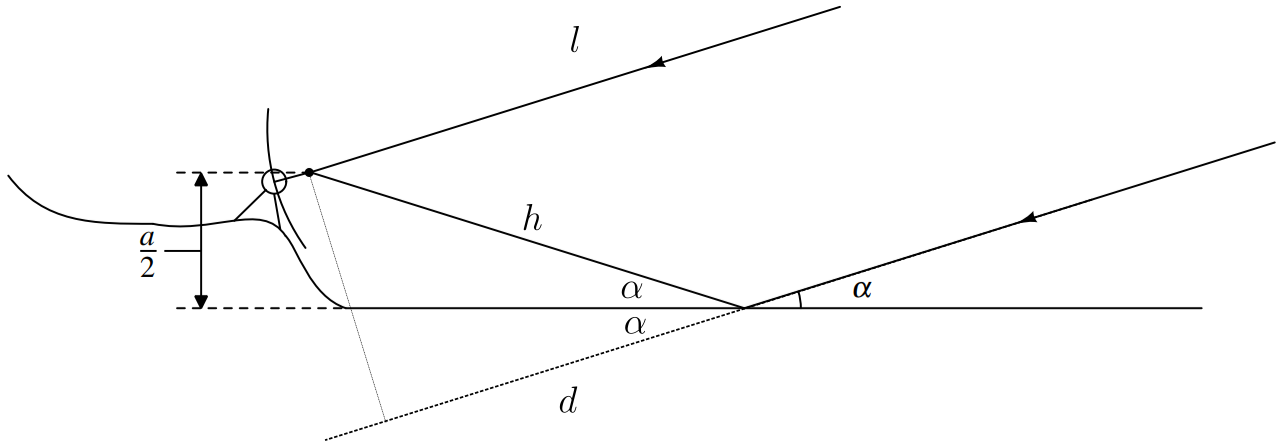
\includegraphics[width=\linewidth]{q4.png}
\end{figure*}

Finding $h$:

\[
    \sin \alpha = \frac{a}{2h} \rightarrow h = \frac{a}{2\sin \alpha}
\]

Now $d$:

\[
    d = h \cos{2 \alpha} = \frac{a \cos{2 \alpha}}{2 \sin \alpha}
\]

Finding the OPL of the lower ray (2nd ray)

\[
    OPL_2 = l - d + h = l - \frac{a \cos{2 \alpha}}{2 \sin \alpha} + \frac{a}{2\sin \alpha} = l + \frac{a}{2\sin \alpha}(1 - \cos{2\alpha}) = l + a \sin \alpha
\]

Now $\Delta OPL$

\[
    \Delta OPL = OPL_2 - OPL_1 = l + a \sin \alpha - l = a \sin \alpha
\]

For the case of multiple beams with ray 2 externally reflecting

\[
    \delta = k \Delta OPL + \pi = ka \sin \alpha + \pi
\]

For multiple beams, we'll have a maximum intensity when $\cos \delta = 1$, so, this occurs when $\delta = 2 \pi n$, where $n\in\mathbb{Z}$:

\[
    ka \sin \alpha + \pi = 2 \pi n
\]

Setting $n=1$ for the first maximum ($n=0$ would be impossible since this would result in $\alpha = 0$):

\[
    ka \sin \alpha = \pi \rightarrow \alpha = \sin^{-1}\left(\frac{\pi}{ka} \right) = \sin^{-1}\left(\frac{\lambda}{2a} \right)
\]


\section*{Question 5}
Determine the general solution to the equation
\[
    \laplacian \varphi = 0
\]
if the universe is restricted to one dimension. (I.e. $\varphi = \varphi(x)$) \\\\

In one dimension, the Laplacian becomes $\dv[2]{x}$

\[
    \dv[2]{\varphi}{x} = 0
\]

One approach to solving this is by finding the characteristic equation to the second order homogenous linear differential equation:

\[
    \lambda^2 = 0
\]

Which has the repeated root $\lambda = 0$. This case of a repeated real root of order 2 gives the following general solution:

\[
    \varphi(x) = e^{\lambda x}(A + Bx) = \fbox{A + Bx}
\]

\section*{Question 6}
A soap film surrounded by air has an index of refraction of 1.34. If a region of the film appears bright
red ($\lambda_0$ = \qty{633}{nm}) in normally reflected light, what is its minimum thickness? \\\\

For normal incidence and when $n_0<n_1<n_2$ (which holds since the soap film is surrounded by air), bright spots satisfy

\[
    2 n_1 d = (m - \frac{1}{2})\lambda
\]

Taking $m=1$ to find the minimum thickness:

\[
    2 n_1 d = \frac{\lambda}{2} \rightarrow d = \frac{\lambda}{4 n_1} = \frac{\qty{633}{nm}}{4(1.34)} = \fbox{\qty{118.1}{nm}}
\]

\section*{Question 7}
A Michelson Interferometer is illuminated with monochromatic light. One of its mirrors is then
moved \qty{2.53e-5}{m}, and it is observed that 92 fringe-pairs, bright and dark, pass by in the process.
Determine the wavelength of the incident beam. \\\\

For a Michelson interferometer surrounded by air,

\[
    2 \Delta d = m \lambda \rightarrow \lambda = \frac{2 \Delta d}{m} = \frac{2 \qty{2.53e-5}{m}}{92} = \qty{5.5e-7}{m}
\]

\section*{Question 8}
Determine the refractive index and thickness of a film to be deposited on a glass surface ($n_g = 1.54$)
such that no normally incident light of wavelength \qty{540}{nm} is reflected. \\

For the consideration of normal incidence and the case of external reflection at both boundaries, destructive interference occurs when 

\[
    2 n_1 d = (m - \frac{1}{2})\lambda
\]

Taking $m=1$ to find the thinnest layer, and since we have 2 free variables, we'll choose $n_1 = 1.33$ so $n_g > n_1$

\[
    2 n_1 d = \frac{\lambda}{2} \rightarrow d = \frac{\lambda}{4 n_1} = \frac{\qty{540}{nm}}{4(1.33)} = \fbox{\qty{105.5}{nm}}
\]

\section*{Question 9}
A glass microscope lens having an index of 1.55 is to be coated with a magnesium fluoride film to
increase the transmission of normally incident yellow light ($\lambda_0 = \qty{550}{nm}$). What minimum thickness
should be deposited on the lens? \\\\

According to the Refractiveindex.info database, $n_{MgF_2} = 1.3777 \approx 1.38$. In the case of $n_0 < n_1 < n_2$, the interference of transmitted light is constructive, so we'll consider the case of $m = 1$ destructive interference of the reflected light, since this will result in the minimum thickness.

\[
    d = \frac{\lambda}{4 n_{MgF_2}} = \frac{\qty{550}{nm}}{4 (1.38)} = \qty{99.64}{nm}
\]




\section*{Question 10}
Solve the differential equation

\[
    {\frac{d^{2}x}{d t^{2}}}-6{\frac{d x}{d t}}+4x=0
\]\\\\

This second order homogenous linear differential equation has the following characteristic equation:

\[
    \lambda^2 - 6\lambda + 4 = 0 \rightarrow \lambda = \frac{6 \pm \sqrt{36 - 16}}{2} = 3 \pm \sqrt{5}
\]

For the case where the characteristic equation has unique real roots $\lambda_1$ and $\lambda_2$, the general solution takes the form of

\[
    x(t) = Ae^{\lambda_1 t} + Be^{\lambda_2 t} = Ae^{(3 - \sqrt{5})t} + Be^{(3 + \sqrt{5})t}
\]








\end{document}